\def\partitiontree{
%\draw[step=0.5,gray,very thin] (0,0) grid (8,5);

\node(top) at (3.5,4.5) { $all{\_}nodes$ };

\node(pvsf) at (2,2.5) { $pvs[false]$ };
\node(pvst) at (5,2.5) { $pvs[true]$ };

\node(p0) at (0.7,0.5) { $p_0$ };
\node(p1) at (1.2,0.5) { $p_1$ };
\node(pd) at (1.6,0.5) { $\ldots$ };
\node(pn) at (2.3,0.5) { $p_{n-1}$ };

\node(s0) at (3.2,0.5) { $s_0$ };
\node(s1) at (3.7,0.5) { $s_1$ };
\node(sd) at (4.1,0.5) { $\ldots$ };
\node(sn) at (4.8,0.5) { $s_{n-1}$ };

\node(g0) at (5.7,0.5) { $g_0$ };
\node(g1) at (6.2,0.5) { $g_1$ };
\node(gd) at (6.6,0.5) { $\ldots$ };
\node(gn) at (7.3,0.5) { $g_{n-1}$ };

\draw[xshift=3.5cm,yshift=3.5cm] (-1,0) -- (1,0)
  node(ptf)[pos=0.25,inner sep=0] {} edge (pvsf.north)
  node[pos=0.5,anchor=south east] {$*$}
  node(ptp)[pos=0.5,inner sep=0] {} edge (top.south)
  node(ptt)[pos=0.75,inner sep=0] {} edge (pvst.north)
  ;

\draw[xshift=1.5cm,yshift=1.5cm] (-1,0) -- (1,0)
  node(pp0)[pos=0.2,inner sep=0] {} edge (p0.north)
  node(pp1)[pos=0.4,inner sep=0] {} edge (p1.north)
  node[pos=0.5,anchor=south east] {$*$}
  node(ppp)[pos=0.5,inner sep=0] {} edge (pvsf.250)
  node(ppn)[pos=0.8,inner sep=0] {} edge (pn.north)
  ;

\draw[xshift=4cm,yshift=1.5cm] (-1,0) -- (1,0)
  node(ps0)[pos=0.2,inner sep=0] {} edge (s0.north)
  node(ps1)[pos=0.4,inner sep=0] {} edge (s1.north)
  node[pos=0.5,anchor=south east] {$*$}
  node(psp)[pos=0.5,inner sep=0] {} edge (pvst.230)
  node(psn)[pos=0.8,inner sep=0] {} edge (sn.north)
  ;

\draw[xshift=6.5cm,yshift=1.5cm] (-1,0) -- (1,0)
  node(pg0)[pos=0.2,inner sep=0] {} edge (g0.north)
  node(pg1)[pos=0.4,inner sep=0] {} edge (g1.north)
  node[pos=0.5,anchor=south east] {}
  node(pgp)[pos=0.5,inner sep=0] {} edge (pvst.310)
  node(pgn)[pos=0.8,inner sep=0] {} edge (gn.north)
  ;
}

\def\partitiongraph{
%\draw[step=0.5,gray,very thin] (0,0) grid (8,5);

\node[cn,s0] (n1) at (0.77,1.27) {};
\node[cn,p0] (n2) at (1.6165,3.3865) {};
\node[cn,s0] (n3) at (2.463,2.54) {};
\node[cn,p0] (n4) at (0.8755,2.54) {};
\node[cn,p2] (n5) at (2.463,0.529) {};
\node[cn,s2] (n6) at (3.945,1.799) {};
\node[cn,s0] (n7) at (3.6275,2.963) {};
\node[cn,p2] (n8) at (4.7915,0.529) {};
\node[cn,s1] (n9) at (5.638,1.5875) {};
\node[cn,s1] (n10) at (6.6965,1.164) {};
\node[cn,s1] (n11) at (5.215,2.6455) {};
\node[cn,p1] (n12) at (6.379,2.7515) {};
\node[cn,p1] (n13) at (5.3205,3.598) {};
\node[cn,s1,g0] (n14) at (4.1565,4.1275) {};
\node[cn,s0] (n15) at (2.8865,3.81) {};
\node[cn,p0] (n16) at (0.77,4.1275) {};
\node[cn,s2,g0] (n17) at (1.405,0.423) {};
\node[cn,p1] (n18) at (6.379,4.0215) {};
\node[cn,s2,g0] (n19) at (2.7805,1.4815) {};
\node[cn,s0] (n20) at (1.7225,1.799) {};
\node[cn,p2] (n21) at (3.733,0.7405) {};
\node[cn,s2] (n22) at (5.85,0.635) {};

\draw (n16) to (n2);
\draw (n16) to (n4);
\draw (n5) to (n21);
\draw (n21) to (n8);
\draw (n12) to (n13) to (n18) to (n12);


\draw[p2s] (n1) to (n4) to (n20);
\draw[p2s] (n4) to (n3) to (n15) to (n2);
\draw[p2s] (n15) to (n7);

\draw[p2s] (n14) to (n13) to (n11) to (n9) to (n12) to (n10);

\draw[p2s] (n17) to (n19) to (n5);
\draw[p2s] (n19) to (n6) to (n8) to (n22);

\draw[s2s] (n1) to (n17);
\draw[s2s] (n20) to (n19) to (n3);
\draw[s2s] (n15) to (n14) to (n7);
\draw[s2s] (n11) to (n6) to (n9) to (n22) to (n10);

\draw[thick] (0.5,0.5) to (4,2.5);
\draw[thick] (3.75,4.5) to (4,2.5);
\draw[thick] (6.5,0.5) to (4,2.5);

\draw[dashed] (0.5,1.5) .. controls (1,2) and (1.5,2.5) .. (1.9,3.1) .. controls (2,4) .. (1.75,4.5);
\draw[dashed] (5.25,4.5) .. controls (4.75,3.5) .. (5.25,3.25) .. controls (6,3) .. (6,2.5) .. controls (6,2.25) .. (7,2.5);
\draw[dashed] (2,0.25) .. controls (2.25,1) .. (3.5,1.1) .. controls (5,1.25) .. (5.5,0.25);
}

\begin{figure}[t]
  \centering
\subfigure[partitioning tree]{
\label{sfig:part_fig:tree}
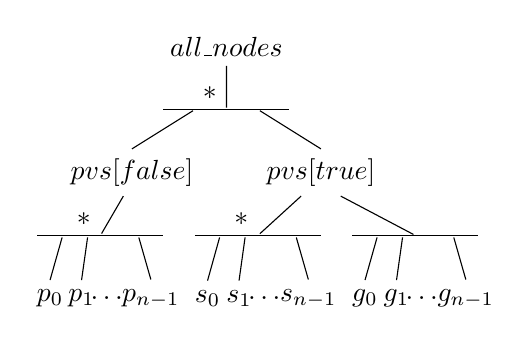
\begin{tikzpicture}[scale=0.8]
\partitiontree
\end{tikzpicture}
}

  \subfigure[$pvs$]{
\label{sfig:part_fig:pvs}
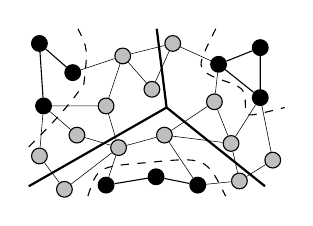
\begin{tikzpicture}
  [scale=0.5, cn/.style={circle,draw,inner sep=0,minimum size=2mm},
   p0/.style={fill},
   p1/.style={fill},
   p2/.style={fill},
   s0/.style={fill=lightgray},
   s1/.style={fill=lightgray},
   s2/.style={fill=lightgray},
   g0/.style={},
   p2p/.style={very thin},
   p2s/.style={very thin},
   s2s/.style={very thin}]
\partitiongraph
\end{tikzpicture}
}
  \subfigure[$p_i$]{
\label{sfig:part_fig:p_i}
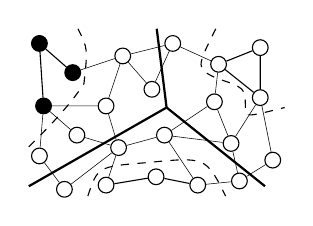
\begin{tikzpicture}
  [scale=0.5, cn/.style={circle,draw,inner sep=0,minimum size=2mm},
   p0/.style={fill},
   p1/.style={},
   p2/.style={},
   s0/.style={},
   s1/.style={},
   s2/.style={},
   g0/.style={},
   p2p/.style={very thin},
   p2s/.style={very thin},
   s2s/.style={very thin}]
\partitiongraph
\end{tikzpicture}
}
  \subfigure[$s_i$]{
\label{sfig:part_fig:s_i}
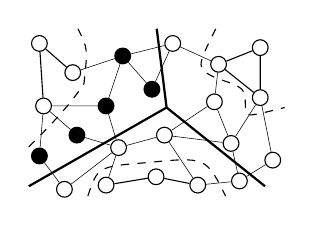
\begin{tikzpicture}
  [scale=0.5, cn/.style={circle,draw,inner sep=0,minimum size=2mm},
   p0/.style={},
   p1/.style={},
   p2/.style={},
   s0/.style={fill},
   s1/.style={},
   s2/.style={},
   g0/.style={},
   p2p/.style={very thin},
   p2s/.style={very thin},
   s2s/.style={very thin}]
\partitiongraph
\end{tikzpicture}
}
  \subfigure[$g_i$]{
\label{sfig:part_fig:g_i}
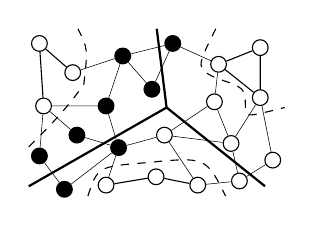
\begin{tikzpicture}
  [scale=0.5, cn/.style={circle,draw,inner sep=0,minimum size=2mm},
   p0/.style={},
   p1/.style={},
   p2/.style={},
   s0/.style={fill},
   s1/.style={},
   s2/.style={},
   g0/.style={fill},
   p2p/.style={very thin},
   p2s/.style={very thin},
   s2s/.style={very thin}]
\partitiongraph
\end{tikzpicture}
}
  \label{fig:part_fig}
  \caption{Partitions of $r{\_}all{\_}nodes$}
%  \caption[My caption
\end{figure}
